\documentclass{article} 
\usepackage{tikz}
\usetikzlibrary{er}
\usepackage{pgffor}
\usetikzlibrary{patterns}
\begin{document}


\begin{tikzpicture}
\draw (-1.5,0) -- (1.5,0);
\draw (0,-1.5) -- (0,1.5);
\end{tikzpicture}



\begin{tikzpicture}
\draw (-1.5,0) -- (1.5,0);
\draw (0,-1.5) -- (0,1.5);
\draw (-1,0) .. controls (-1,0.555) and (-0.555,1) .. (0,1)
.. controls (0.555,1) and (1,0.555) .. (1,0);
\end{tikzpicture}


\tikz \draw (0,0) circle (10pt);



\tikz \draw (0,0) ellipse (20pt and 10pt);



\begin{tikzpicture}
\draw (-1.5,0) -- (1.5,0);
\draw (0,-1.5) -- (0,1.5);
\draw (0,0) circle (1cm);
\end{tikzpicture}




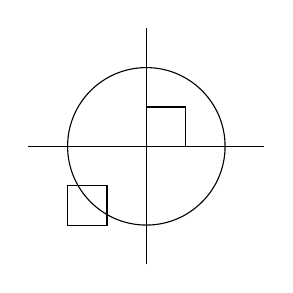
\begin{tikzpicture}
\draw (-1.5,0) -- (1.5,0);
\draw (0,-1.5) -- (0,1.5);
\draw (0,0) circle (1cm);
\draw (0,0) rectangle (0.5,0.5);
\draw (-0.5,-0.5) rectangle (-1,-1);
\end{tikzpicture}



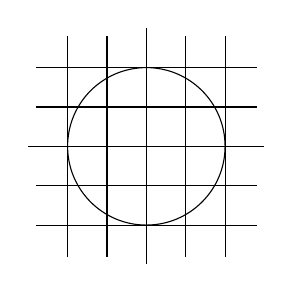
\begin{tikzpicture}
\draw (-1.5,0) -- (1.5,0);
\draw (0,-1.5) -- (0,1.5);
\draw (0,0) circle (1cm);
\draw[step=.5cm] (-1.4,-1.4) grid (1.4,1.4);
\end{tikzpicture}




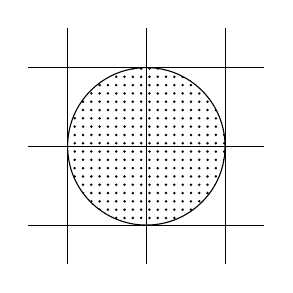
\begin{tikzpicture}
\draw (-1.5,0) -- (1.5,0);
\draw (0,-1.5) -- (0,1.5);
\draw[pattern=dots] (0,0) circle (1cm);
\draw[step=1cm] (-1.5,-1.5) grid (1.5,1.5);
\end{tikzpicture}





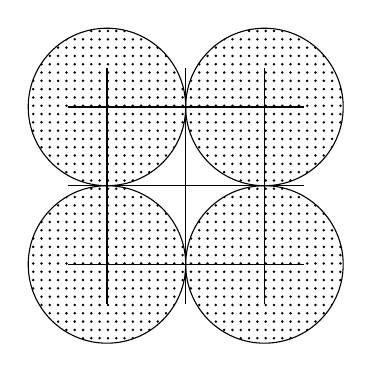
\begin{tikzpicture}
%\draw (-1.5,0) -- (1.5,0);
%\draw (0,-1.5) -- (0,1.5);
\draw[pattern=dots] (-1,-1) circle (1cm);
\draw[pattern=dots] (1,-1) circle (1cm);
\draw[pattern=dots] (-1,1) circle (1cm);
\draw[pattern=dots] (1,1) circle (1cm);
\draw[step=1cm] (-1.5,-1.5) grid (1.5,1.5);
\end{tikzpicture}


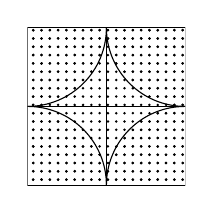
\begin{tikzpicture}
%\draw (-1.5,0) -- (1.5,0);
%\draw (0,-1.5) -- (0,1.5);
\clip (-1,-1) rectangle (1,1);
\draw[pattern=dots] (-1,-1) rectangle (1,1);
\draw[pattern=dots] (-1,-1) circle (1cm);
\draw[pattern=dots] (1,-1) circle (1cm);
\draw[pattern=dots] (-1,1) circle (1cm);
\draw[pattern=dots] (1,1) circle (1cm);
\draw[step=1cm] (-1.5,-1.5) grid (1.5,1.5);
\end{tikzpicture}



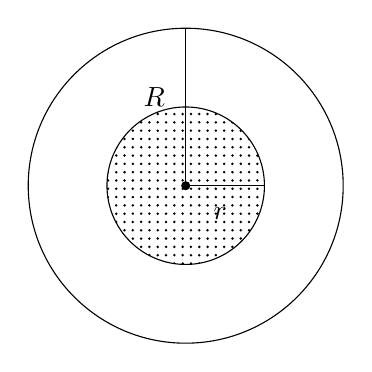
\begin{tikzpicture}
\draw (0,0) -- (0,2) node[below=25pt,left=4pt,fill=white] {$R$};
\draw (0,0) -- (1,0) node[below=10pt,left=10pt,fill=white] {$r$};
\draw (0,0) circle (2cm);
\draw[pattern=dots] (0,0) circle (1cm);
\filldraw[color=black] (0,0) circle (.05cm);
\end{tikzpicture}




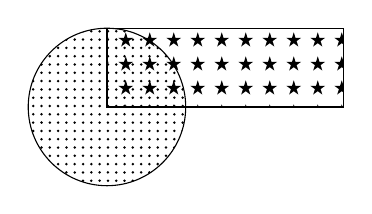
\begin{tikzpicture}
\draw[pattern=dots] (0,0) circle (1cm);
\draw[pattern=fivepointed stars] (0,0) rectangle (3,1);
\end{tikzpicture}






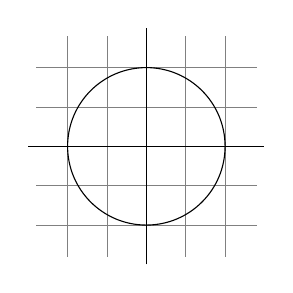
\begin{tikzpicture}
\draw[step=.5cm,gray,very thin] (-1.4,-1.4) grid (1.4,1.4);
\draw (-1.5,0) -- (1.5,0);
\draw (0,-1.5) -- (0,1.5);
\draw (0,0) circle (1cm);
\end{tikzpicture}





\tikz \draw (0,0) arc (0:215:1.75cm and 1cm);


\tikz \draw (0,0) rectangle (1,1) (0,0) parabola (1,1);



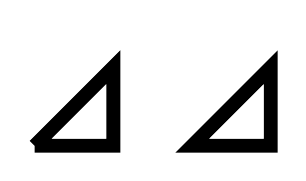
\begin{tikzpicture}[line width=5pt]
\draw (0,0) -- (1,0) -- (1,1) -- (0,0);
\draw (2,0) -- (3,0) -- (3,1) -- cycle;
\useasboundingbox (0,1.5); % make bounding box higher
\end{tikzpicture}




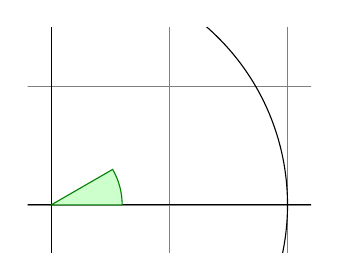
\begin{tikzpicture}[scale=3]
\clip (-0.1,-0.2) rectangle (1.1,0.75);
\draw[step=.5cm,gray,very thin] (-1.4,-1.4) grid (1.4,1.4);
\draw (-1.5,0) -- (1.5,0);
\draw (0,-1.5) -- (0,1.5);
\draw (0,0) circle (1cm);
\filldraw[fill=green!20!white, draw=green!50!black]
(0,0) -- (3mm,0mm) arc (0:30:3mm) -- cycle;
\end{tikzpicture}



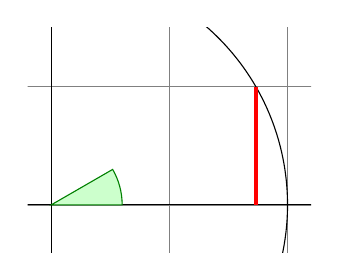
\begin{tikzpicture}[scale=3]
\clip (-0.1,-0.2) rectangle (1.1,0.75);
\draw[step=.5cm,gray,very thin] (-1.4,-1.4) grid (1.4,1.4);
\draw (-1.5,0) -- (1.5,0);
\draw (0,-1.5) -- (0,1.5);
\draw (0,0) circle (1cm);
\filldraw[fill=green!20,draw=green!50!black]
(0,0) -- (3mm,0mm) arc (0:30:3mm) -- cycle;
\draw[red,very thick] (30:1cm) -- +(0,-0.5);
\end{tikzpicture}





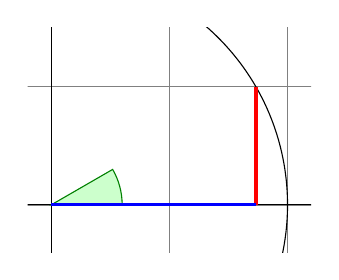
\begin{tikzpicture}[scale=3]
\clip (-0.1,-0.2) rectangle (1.1,0.75);
\draw[step=.5cm,gray,very thin] (-1.4,-1.4) grid (1.4,1.4);
\draw (-1.5,0) -- (1.5,0);
\draw (0,-1.5) -- (0,1.5);
\draw (0,0) circle (1cm);
\filldraw[fill=green!20,draw=green!50!black] (0,0) -- (3mm,0mm) arc
(0:30:3mm) -- cycle;
\draw[red,very thick] (30:1cm) -- +(0,-0.5);
\draw[blue,very thick] (30:1cm) ++(0,-0.5) -- (0,0);
\end{tikzpicture}





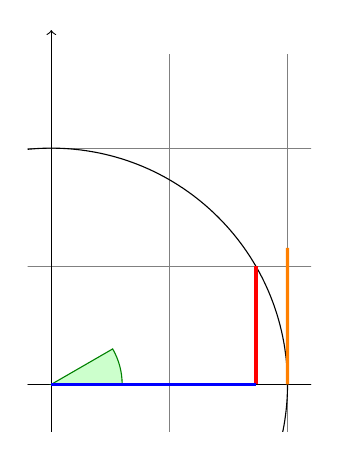
\begin{tikzpicture}[scale=3]
\clip (-0.1,-0.2) rectangle (1.1,1.51);
\draw[step=.5cm,gray,very thin] (-1.4,-1.4) grid (1.4,1.4);
\draw[->] (-1.5,0) -- (1.5,0);
\draw[->] (0,-1.5) -- (0,1.5);
\draw (0,0) circle (1cm);
\filldraw[fill=green!20,draw=green!50!black] (0,0) -- (3mm,0mm) arc
(0:30:3mm) -- cycle;
\draw[red,very thick] (30:1cm) -- +(0,-0.5);
\draw[blue,very thick] (30:1cm) ++(0,-0.5) -- (0,0);
\draw[orange,very thick] (1,0) -- (intersection of 1,0--1,1 and 0,0--30:1cm);
\end{tikzpicture}





\tikz \foreach \x in {1,...,10}
	\draw (\x,0) circle (0.4cm);





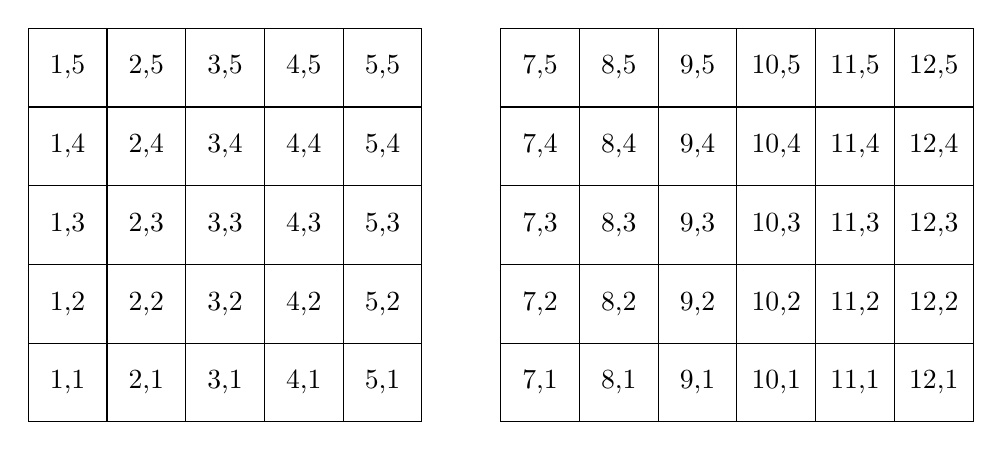
\begin{tikzpicture}
\foreach \x in {1,2,...,5,7,8,...,12}
\foreach \y in {1,...,5}
{
\draw (\x,\y) +(-.5,-.5) rectangle ++(.5,.5);
\draw (\x,\y) node{\x,\y};
}
\end{tikzpicture}





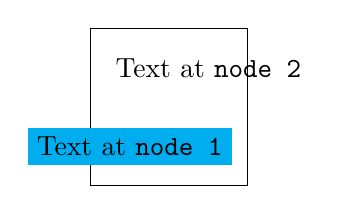
\begin{tikzpicture}
\draw (0,0) rectangle (2,2);
\draw (0.5,0.5) node [fill=cyan]
{Text at \verb!node 1!};
\draw (1.5,1.5) node {Text at \verb!node 2!};
\end{tikzpicture}






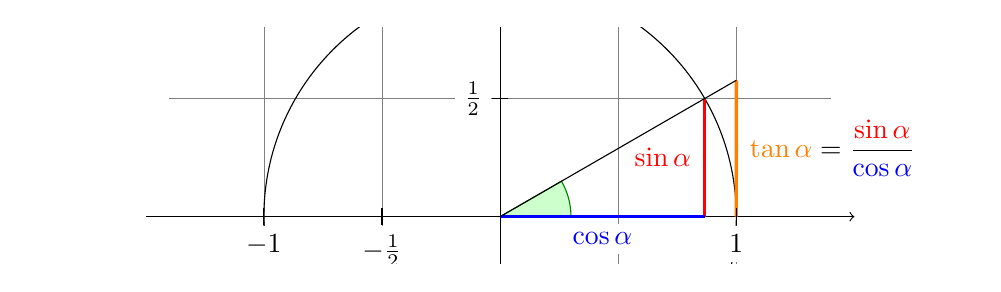
\begin{tikzpicture}[scale=3]
\clip (-2,-0.2) rectangle (2,0.8);
\draw[step=.5cm,gray,very thin] (-1.4,-1.4) grid (1.4,1.4);
\filldraw[fill=green!20,draw=green!50!black] (0,0) -- (3mm,0mm) arc
(0:30:3mm) -- cycle;
\draw[->] (-1.5,0) -- (1.5,0) coordinate (x axis);
\draw[->] (0,-1.5) -- (0,1.5) coordinate (y axis);
\draw (0,0) circle (1cm);
\draw[very thick,red]
(30:1cm) -- node[left=1pt,fill=white] {$\sin \alpha$} (30:1cm |- x axis);
\draw[very thick,blue]
(30:1cm |- x axis) -- node[below=2pt,fill=white] {$\cos \alpha$} (0,0);
\draw[very thick,orange] (1,0) -- node [right=1pt,fill=white]
{$\displaystyle \tan \alpha \color{black}=
\frac{{\color{red}\sin \alpha}}{\color{blue}\cos \alpha}$}
(intersection of 0,0--30:1cm and 1,0--1,1) coordinate (t);
\draw (0,0) -- (t);
\foreach \x/\xtext in {-1, -0.5/-\frac{1}{2}, 1}
\draw (\x cm,1pt) -- (\x cm,-1pt) node[anchor=north,fill=white] {$\xtext$};
\foreach \y/\ytext in {-1, -0.5/-\frac{1}{2}, 0.5/\frac{1}{2}, 1}
\draw (1pt,\y cm) -- (-1pt,\y cm) node[anchor=east,fill=white] {$\ytext$};
\end{tikzpicture}







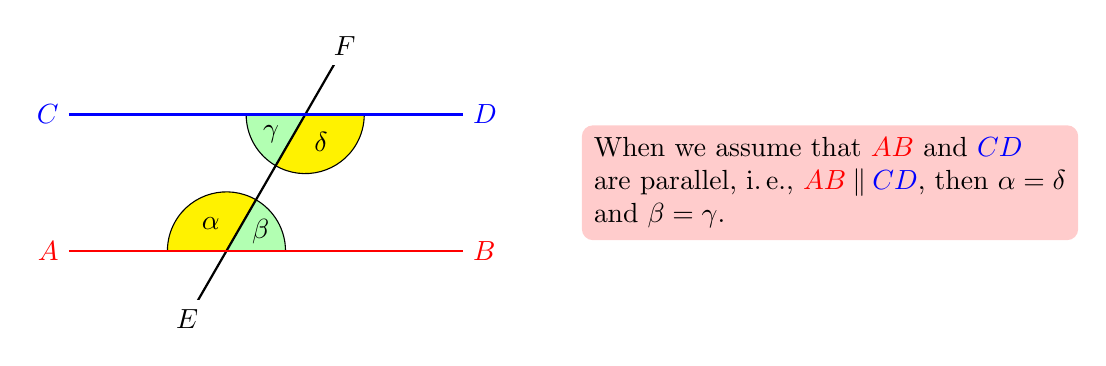
\begin{tikzpicture}
\draw[fill=yellow] (0,0) -- (60:.75cm) arc (60:180:.75cm);
\draw(120:0.4cm) node {$\alpha$};
\draw[fill=green!30] (0,0) -- (right:.75cm) arc (0:60:.75cm);
\draw(30:0.5cm) node {$\beta$};
\begin{scope}[shift={(60:2cm)}]
\draw[fill=green!30] (0,0) -- (180:.75cm) arc (180:240:.75cm);
\draw (30:-0.5cm) node {$\gamma$};
\draw[fill=yellow] (0,0) -- (240:.75cm) arc (240:360:.75cm);
\draw (-60:0.4cm) node {$\delta$};
\end{scope}
\begin{scope}[thick]
\draw (60:-1cm) node[fill=white] {$E$} -- (60:3cm) node[fill=white] {$F$};
\draw[red] (-2,0) node[left] {$A$} -- (3,0) node[right]{$B$};
\draw[blue,shift={(60:2cm)}] (-3,0) node[left] {$C$} -- (2,0) node[right]{$D$};
\draw[shift={(60:1cm)},xshift=4cm]
node [right,text width=6cm,rounded corners,fill=red!20,inner sep=1ex]
{
When we assume that $\color{red}AB$ and $\color{blue}CD$ are
parallel, i.\,e., ${\color{red}AB} \mathbin{\|} \color{blue}CD$,
then $\alpha = \delta$ and $\beta = \gamma$.
};
\end{scope}
\end{tikzpicture}





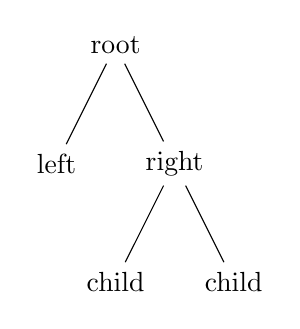
\begin{tikzpicture}
\node {root}
child {node {left}}
child {node {right}
child {node {child}}
child {node {child}}
};
\end{tikzpicture}







\begin{tikzpicture}[->]
\draw (0,0) -- (1,0);
\draw (0,0) -- (0,1,0);
\draw (0,0) -- (0,0,1);
\end{tikzpicture}





\begin{tikzpicture}[->]
\draw (0,0) -- (3,0);
\draw (0,0) -- (0,3,0);
\draw (0,0) -- (0,0,3);
\end{tikzpicture}






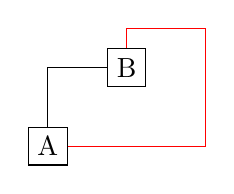
\begin{tikzpicture}
\draw (0,0) node(a) [draw] {A} (1,1) node(b) [draw] {B};
\draw (a.north) |- (b.west);
\draw[color=red] (a.east) -| (2,1.5) -| (b.north);
\end{tikzpicture}




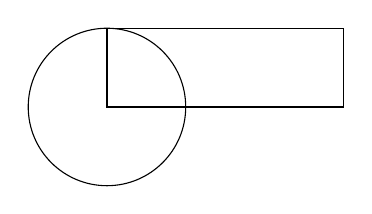
\begin{tikzpicture}
\draw (0,0) circle (1cm);
\draw (0,0) rectangle (3,1);
\end{tikzpicture}





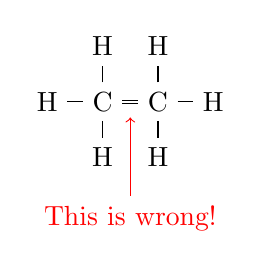
\begin{tikzpicture}[level distance=2em]
\node {C}
child[grow=up] {node {H}}
child[grow=left] {node {H}}
child[grow=down] {node {H}}
child[grow=right] {node {C}
child[grow=up] {node {H}}
child[grow=right] {node {H}}
child[grow=down] {node {H}}
edge from parent[double]
coordinate (wrong)
};
\draw[<-,red] ([yshift=-2mm]wrong) -- +(0,-1)
node[below]{This is wrong!};
\end{tikzpicture}






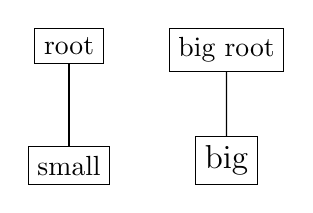
\begin{tikzpicture}[level distance=2cm,growth parent anchor=north]
\tikzstyle{every node}=[anchor=north,rectangle,draw]
\tikzstyle{every child node}=[anchor=south]
\node at (0,0) {root} child {node {small}};
\node at (2,0) {big root} child {node {\large big}};
\end{tikzpicture}




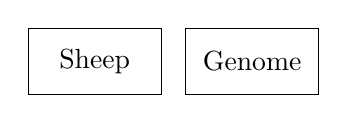
\begin{tikzpicture}[node distance=2cm]
\node[entity] (sheep) {Sheep};
\node[entity] (genome) [right of=sheep] {Genome};
\end{tikzpicture}




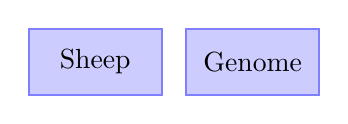
\begin{tikzpicture}[node distance=2cm]
\tikzstyle{every entity}=[draw=blue!50,fill=blue!20,thick]
\node[entity] (sheep) {Sheep};
\node[entity] (genome) [right of=sheep] {Genome};
\end{tikzpicture}




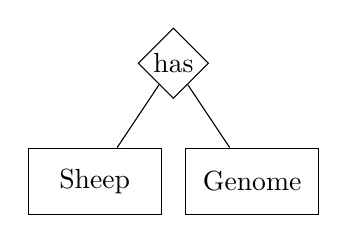
\begin{tikzpicture}
\node[entity] (sheep) at (0,0) {Sheep};
\node[entity] (genome) at (2,0) {Genome};
\node[relationship] at (1,1.5) {has}
edge (sheep)
edge (genome);
\end{tikzpicture}




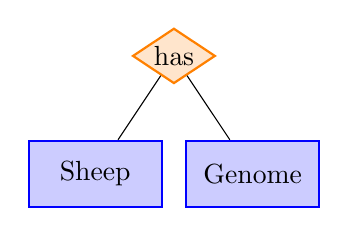
\begin{tikzpicture}
\tikzstyle{every entity}=[fill=blue!20,draw=blue,thick]
\tikzstyle{every relationship}=[fill=orange!20,draw=orange,thick,aspect=1.5]
\node[entity] (sheep) at (0,0) {Sheep};
\node[entity] (genome) at (2,0) {Genome};
\node[relationship] at (1,1.5) {has}
edge (sheep)
edge (genome);
\end{tikzpicture}






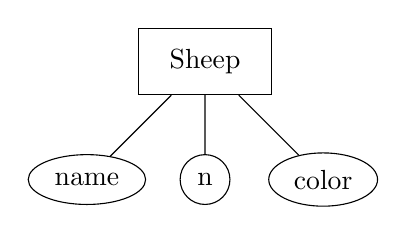
\begin{tikzpicture}
\node[entity] (sheep) {Sheep}
child {node[attribute] {name}}
child {node[attribute] {n}}
child {node[attribute] {color}};
\end{tikzpicture}




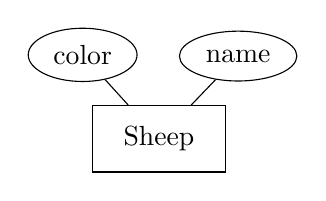
\begin{tikzpicture}
\tikzstyle{every pin edge}=[draw]
\node[entity,pin={[attribute]60:name},pin={[attribute]120:color}] {Sheep};
\end{tikzpicture}






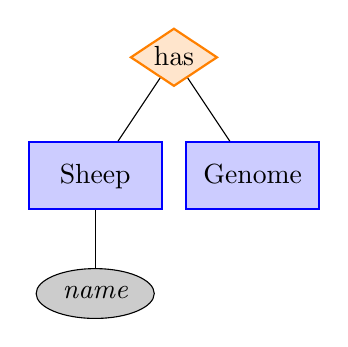
\begin{tikzpicture}[text depth=1pt]
\tikzstyle{every attribute}=[fill=black!20,draw=black]
\tikzstyle{every entity}=[fill=blue!20,draw=blue,thick]
\tikzstyle{every relationship}=[fill=orange!20,draw=orange,thick,aspect=1.5]
\node[entity] (sheep) at (0,0) {Sheep}
child {node [key attribute] {name}};
\node[entity] (genome) at (2,0) {Genome};
\node[relationship] at (1,1.5) {has}
edge (sheep)
edge (genome);
\end{tikzpicture}






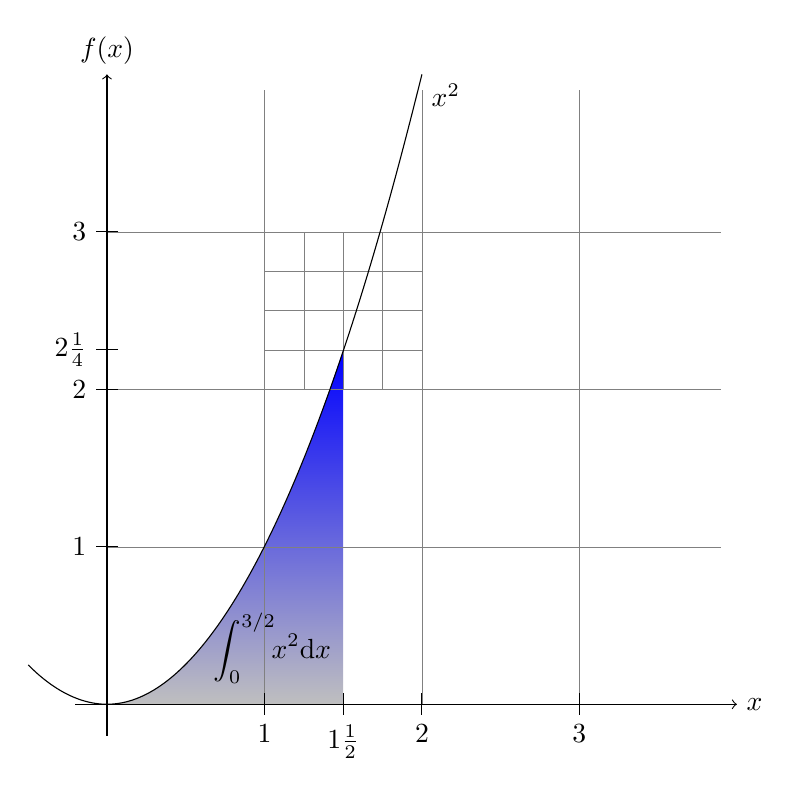
\begin{tikzpicture}[scale=2]
\shade[top color=blue,bottom color=gray!50] (0,0) parabola (1.5,2.25) |- (0,0);
\draw (1.05cm,2pt) node[above] {$\displaystyle\int_0^{3/2} \!\!x^2\mathrm{d}x$};
\draw[style=help lines] (0,0) grid (3.9,3.9)
[step=0.25cm] (1,2) grid +(1,1);
\draw[->] (-0.2,0) -- (4,0) node[right] {$x$};
\draw[->] (0,-0.2) -- (0,4) node[above] {$f(x)$};
\foreach \x/\xtext in {1/1, 1.5/1\frac{1}{2}, 2/2, 3/3}
\draw[shift={(\x,0)}] (0pt,2pt) -- (0pt,-2pt) node[below] {$\xtext$};
\foreach \y/\ytext in {1/1, 2/2, 2.25/2\frac{1}{4}, 3/3}
\draw[shift={(0,\y)}] (2pt,0pt) -- (-2pt,0pt) node[left] {$\ytext$};
\draw (-.5,.25) parabola bend (0,0) (2,4) node[below right] {$x^2$};
\end{tikzpicture}





\foreach \x in {1,2,3,0} {[\x]}


\tikz
\foreach \x in {0,1,2,3}
\draw (\x,0) circle (0.2cm);





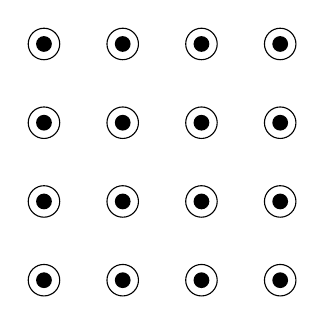
\begin{tikzpicture}
\foreach \x in {0,1,2,3}
\foreach \y in {0,1,2,3}
{
\draw (\x,\y) circle (0.2cm);
\fill (\x,\y) circle (0.1cm);
}
\end{tikzpicture}





\tikz
\foreach \position in {(0,0), (1,1), (2,0), (3,1)}
\draw \position rectangle +(.25,.5);




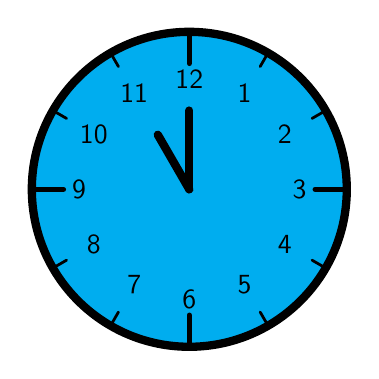
\begin{tikzpicture}[cap=round,line width=3pt]
\filldraw [fill=cyan] (0,0) circle (2cm);
\foreach \angle / \label in
{0/3, 30/2, 60/1, 90/12, 120/11, 150/10, 180/9,
210/8, 240/7, 270/6, 300/5, 330/4}
{
\draw[line width=1pt] (\angle:1.8cm) -- (\angle:2cm);
\draw (\angle:1.4cm) node{\textsf{\label}};
}
\foreach \angle in {0,90,180,270}
\draw[line width=2pt] (\angle:1.6cm) -- (\angle:2cm);
\draw (0,0) -- (120:0.8cm); % hour
\draw (0,0) -- (90:1cm); % minute
\end{tikzpicture}











\end{document}